\chapter{容器化环境中的横向移动时空特性分析}{
{
\let\cleardoublepage\relax
}
\label{chap:embedding}

% 为了通过网络流量来检测容器化环境中的横向移动,我们需要了解横向移动的原理,以及横向移动在网络流量特征中的表现。本章将首先介绍横向移动的原理,讨论容器化环境中横向移动的特点,分析横向移动流量与良性流量的特征差异,然后在数据集上进行特征分析,最后使用决策树和互信息量检验,进行特征重要度评估。

横向移动除了导致流量的特征与良性流量相比有所不同以外,还会对网络的拓扑结构产生影响;此外,也会对网络流量随时间的变化产生影响。

本文研究和分析了容器化环境中的网络流量拓扑结构,发现横向移动行为会导致网络流量拓扑结构发生改变。例如,攻击者发起横向移动攻击后,从未与 API 服务器通信的负载开始与 API 服务器通信。因此,通过检测拓扑结构的变化可以检测出关键的横向移动流量。

对于大多数横向移动流量,本文进行了空间特征嵌入方法和时间特征嵌入方法研究,进一步挖掘网络流量中包含的信息,得到空间和时间特征嵌入向量,用于后续模型的输入。

\section{横向移动对网络流量拓扑结构的影响}
\label{sec:topology}

容器化环境中的网络流量服从一定的规律,可以从中挖掘一定的空间特征。如果将流量建模为图,图上的节点代表 IP 地址和端口的组合\footnote{IP 地址相同、端口号大于 32768 的,聚合为同一个节点。},边代表节点之间产生的流量,便可以利用图机器学习的方式挖掘这些空间特征,并通过节点的嵌入向量表现出来。

从第~\ref{sec:theory}~节的分析,可以看到,当攻击者侵入容器化集群中的负载之后,他可能移动到其他负载、主机等地方,并且将该负载与攻击者的 C\&C 服务器建立连接,以便部署恶意软件并进行控制。因此,横向移动会导致网络流量拓扑结构发生如下改变:

\begin{itemize}
    \item 负载与 API 服务器之间的连接关系发生变化。正常情况下不需要与 API 服务器通信的负载在遭受攻击后开始与 API 服务器通信,以便获取集群的配置文件并执行资源操作。
    \item 负载之间的连接关系发生变化。正常情况下不需要通信的负载之间发生通信,这表明攻击者在负载之间进行了横向移动。
    \item 容器化集群中出现了新的负载,且该负载与集群配置的扩容策略等无关。这种情况说明,攻击者通过 API 服务器非法创建了一个新的负载,该负载可能带有特殊权限,以便攻击者从负载移动到主机上。
    \item 负载与外部网络之间的连接关系发生变化。当正常情况下不需要与外部网络通信的负载开始与外部网络通信时,或者负载开始访问其以前从未访问过的网段时,说明该负载被攻击者控制,并与攻击者的 C\&C 服务器通信。
    \item 主机与外部网络之间的连接关系发生变化。和上述情况类似,当攻击者从负载移动到主机上时,主机将开始处于攻击者的 C\&C 服务器之下。
\end{itemize}

\section{网络流量的拓扑结构分析}
\label{sec:topology}

为了更加具体地研究横向移动对网络流量拓扑结构的影响,本文继续在 Kubernetes-dataset 数据集上进行分析,数据集的详细介绍见第~\ref{sec:dataset}~节。

首先,将数据集中的良性流建模为图,然后通过 NetworkX\citep{networkx} 可视化,如图~\ref{fig:benign-structure}~所示。

\begin{figure}[t]
    \centering
    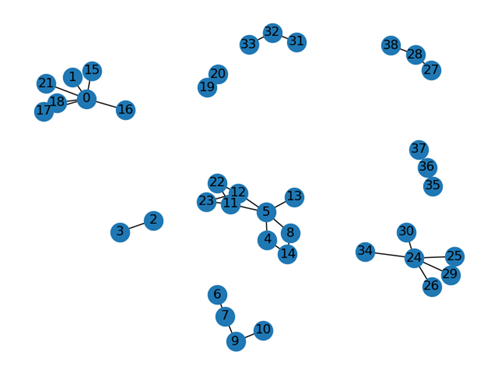
\includegraphics[width=0.75\textwidth]{benign-structure}
    \bicaption{\enspace 良性流的网络拓扑结构}{\enspace Topological diagram of benign flows}
    \label{fig:benign-structure}

\end{figure}

可以看到,在容器化集群中,各节点分为 9 个组,并在组内进行通信,这些通信表现出了不同的通信模式。接下来对不同的通信模式进行分析。

(一)主机与负载之间的通信。节点 0、1、15、16、17、18、21 之间的通信属于此类。这些节点的 IP 地址和端口如表~\ref{tab:benign-structure-1}~所示。

\begin{table}[!htbp]
    \bicaption{\enspace 良性流中主机与负载之间通信的相关节点}{\enspace Nodes related to communications between hosts and pods}
    \label{tab:benign-structure-1}
    \centering
    \footnotesize% fontsize
    \setlength{\tabcolsep}{4pt}% column separation
    \renewcommand{\arraystretch}{1.2}%row space 
    \begin{tabular}{cccccc}
        \hline
        编号 & IP 地址 & 端口\\
        \hline
        0 & 100.64.0.2 & \geq 32768\\
        1 & 10.16.0.45 & 1880\\
        15 & 10.16.0.5 & 8080\\
        16 & 10.16.0.4 & 8181\\
        17 & 10.16.0.4 & 8080\\
        18 & 10.16.0.7 & 7472\\
        21 & 10.16.0.5 & 8181\\
        \hline
    \end{tabular}
\end{table}

在这些节点中,节点 0 为主机节点,其余节点为负载节点。其中,节点 16、17 和 15、18 分别部署了 HTTP 服务,节点 1 部署了 Node-RED 服务,节点 18 部署了其他服务。主机是以客户端的身份向这些负载通信的,也就是说这些流量代表了对负载中部署的应用程序的访问。

(二)API 服务器与负载之间的通信。节点 4、5、8、11、12、13 之间的通信属于此类。这些节点的 IP 地址和端口如表~\ref{tab:benign-structure-2}~所示。

\begin{table}[!htbp]
    \bicaption{\enspace 良性流中 API 服务器与负载之间通信的相关节点}{\enspace Nodes related to communications between the API server and pods}
    \label{tab:benign-structure-2}
    \centering
    \footnotesize% fontsize
    \setlength{\tabcolsep}{4pt}% column separation
    \renewcommand{\arraystretch}{1.2}%row space 
    \begin{tabular}{cccccc}
        \hline
        编号 & IP 地址 & 端口\\
        \hline
        4 & 10.16.0.2 & \geq 32768\\
        5 & 144.122.71.18 & 6443\\
        8 & 10.16.0.6 & \geq 32768\\
        11 & 10.16.0.5 & \geq 32768\\
        12 & 10.16.0.4 & \geq 32768\\
        13 & 10.16.0.7 & \geq 32768\\
        \hline
    \end{tabular}
\end{table}

通过端口号和 IP 地址,可以看出,节点 5 为 API 服务器节点,其他节点为负载节点,并且这些负载主动向 API 服务器发起连接。这些通信表示负载节点正在使用 API 服务器提供的服务,这些服务可用于获取负载和集群的配置、修改集群的资源等。

(三)负载与外部网络的通信。节点 19、20,节点 24、25、26、29、30、34,节点 31、32、33 之间的通信属于此类。这些节点的 IP 地址和端口如表~\ref{tab:benign-structure-3}~所示。

\begin{table}[!htbp]
    \bicaption{\enspace 良性流中负载与外部网络之间通信的相关节点}{\enspace Nodes related to communications between pods and external network}
    \label{tab:benign-structure-3}
    \centering
    \footnotesize% fontsize
    \setlength{\tabcolsep}{4pt}% column separation
    \renewcommand{\arraystretch}{1.2}%row space 
    \begin{tabular}{cccccc}
        \hline
        编号 & IP 地址 & 端口\\
        \hline
        19 & 10.16.0.9 & \geq 32768\\
        20 & 18.165.61.116 & 443\\
        24 & 10.16.0.18 & \geq 32768\\
        25 & 34.120.177.193 & 443\\
        26 & 185.199.111.133 & 443\\
        29 & 185.199.108.133 & 443\\
        30 & 108.199.110.133 & 443\\
        31 & 10.16.0.14 & \geq 32768\\
        32 & 62.12.173.11 & 123\\
        33 & 10.16.0.12 & \geq 32768\\
        34 & 185.199.109.133 & 443\\
        \hline
    \end{tabular}
\end{table}

从 IP 地址和端口号可以看出,节点 19、24、31、33 为负载节点,其他节点为外部网络节点,负载节点向外部节点请求资源。在这些外部节点中,有一个节点提供网络时钟服务,其他节点提供 HTTPS 服务。

(四)DNS 通信。节点 22、23 与节点 11、12 之间,节点 27、28、38 之间的通信属于此类。这些节点的 IP 地址和端口如表~\ref{tab:benign-structure-4}~所示,其中,节点 11、12 已在表~\ref{tab:benign-structure-2}~中出现过,不再重复展示。

\begin{table}[!htbp]
    \bicaption{\enspace 良性流中与 DNS 通信相关的节点}{\enspace Nodes related to DNS communications}
    \label{tab:benign-structure-4}
    \centering
    \footnotesize% fontsize
    \setlength{\tabcolsep}{4pt}% column separation
    \renewcommand{\arraystretch}{1.2}%row space 
    \begin{tabular}{cccccc}
        \hline
        编号 & IP 地址 & 端口\\
        \hline
        22 & 144.122.171.92 & 53\\
        23 & 144.122.171.91 & 53\\
        27 & 10.16.0.4 & 53\\
        28 & 144.122.171.92 & \geq 32768\\
        38 & 100.64.0.5 & 53\\
        \hline
    \end{tabular}
\end{table}

(五)网络层或数据链路层的通信。节点 2、3,节点 6、7、9、10 之间的通信属于此类,这些节点的 IP 地址和端口如表~~\ref{tab:benign-structure-5}~~所示。

\begin{table}[!htbp]
    \bicaption{\enspace 良性流中与网络层或数据链路层通信相关的节点}{\enspace Nodes related to Layer 2 or 3 communications of TCP/IP stack}
    \label{tab:benign-structure-5}
    \centering
    \footnotesize% fontsize
    \setlength{\tabcolsep}{4pt}% column separation
    \renewcommand{\arraystretch}{1.2}%row space 
    \begin{tabular}{cccccc}
        \hline
        编号 & IP 地址 & 端口\\
        \hline
        2 & 100.64.0.2 & 0\\
        3 & 100.64.0.1 & 0\\
        6 & 10.16.0.2 & 0\\
        7 & 144.122.71.18 & 0\\
        9 & 10.16.0.6 & 0\\
        10 & 114.114.114.114 & 0\\
        \hline
    \end{tabular}
\end{table}

由于没有进行传输层(TCP、UDP)的通信,因此其端口号记为 0。此类通信可能是 ICMP 或 ARP 通信。

(六)设备发现通信。节点 35、36、37 之间的通信属于此类,这些节点的 IP 地址和端口如表~\ref{tab:benign-structure-6}~所示。

\begin{table}[!htbp]
    \bicaption{\enspace 良性流中与设备发现通信相关的节点}{\enspace Nodes related to communications of device discovery}
    \label{tab:benign-structure-6}
    \centering
    \footnotesize% fontsize
    \setlength{\tabcolsep}{4pt}% column separation
    \renewcommand{\arraystretch}{1.2}%row space 
    \begin{tabular}{cccccc}
        \hline
        编号 & IP 地址 & 端口\\
        \hline
        35 & 100.64.0.2 & 5353\\
        36 & 224.0.0.251 & 5353\\
        37 & 100.64.0.5 & 5353\\
        \hline
    \end{tabular}
\end{table}

从 IP 地址可以发现,节点 35、37 为主机节点,节点 36 为组播地址。该通信可能用于查找打印机、共享文件夹等资源。

(七)Kube-OVN 相关通信。节点 14 的 IP 地址为 144.122.71.18,端口号为 6642,为 Kube-OVN 监听节点。Kube-OVN 插件是用于构建容器化集群的子网,以便抓取数据包并生成数据集。

分析了这些节点的通信模式之后,把横向移动流也加入进来,所有流量的拓扑图如图~\ref{fig:all-structure}~所示。

\begin{figure}[!htbp]
    \centering
    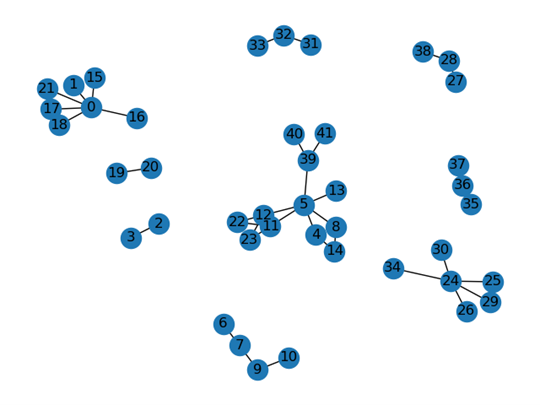
\includegraphics[width=0.75\textwidth]{all-structure}
    \bicaption{\enspace 所有流的网络拓扑结构}{\enspace Topological diagram of all flows}
    \label{fig:all-structure}

\end{figure}

与图~\ref{fig:benign-structure}~相比,图~\ref{fig:all-structure}~增加了三个节点,这些节点的 IP 地址和端口如表~\ref{tab:all-structure}~所示。

\begin{table}[t]
    \bicaption{\enspace 横向移动流中新增的节点}{\enspace Nodes added in malicious flows}
    \label{tab:all-structure}
    \centering
    \footnotesize% fontsize
    \setlength{\tabcolsep}{4pt}% column separation
    \renewcommand{\arraystretch}{1.2}%row space 
    \begin{tabular}{cccccc}
        \hline
        编号 & IP 地址 & 端口\\
        \hline
        39 & 10.16.0.45 & \geq 32768\\
        40 & 144.122.71.36 & 9001\\
        41 & 95.179.254.105 & 443\\
        \hline
    \end{tabular}
\end{table}

注意到节点 39 与节点 1 共享同一个 IP 地址,这表示它们均为 Node-RED 节点。部署 Node-RED 的负载本身无需与 API 服务器通信,但是在攻击者利用了 Node-RED 的漏洞之后,Node-RED 就会不同寻常地与 API 服务器通信,同时还与外部网络进行通信。这说明此时 Node-RED 很可能处于攻击者的 C\&C 服务器的控制之下。因此,这些节点对应的 $7$ 个流是横向移动的关键流。

最后,考虑仅包括横向移动流量的拓扑结构,如图~\ref{fig:malicious-structure}~所示。

\begin{figure}[t]
    \centering
    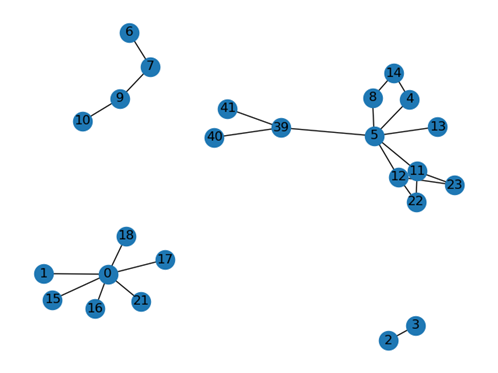
\includegraphics[width=0.75\textwidth]{malicious-structure}
    \bicaption{\enspace 横向移动流的网络拓扑结构}{\enspace Topological diagram of malicious flows}
    \label{fig:malicious-structure}

\end{figure}

从图~\ref{fig:malicious-structure}~可以看出,第(六)类通信即设备发现通信没有出现,说明设备发现通信与横向移动无关,因此可以将其从数据集中删除。

通过上述分析,本文发现,在数据集所提供的横向移动场景中,以往从未与 API 服务器和外部网络通信的 Node-RED 负载开始与 API 服务器和外部网络通信。这说明,攻击者侵入 Node-RED 负载之后,将该负载置于攻击者的 C\&C 服务器之下,并且在该负载上向 API 服务器发起非法请求,使其创建一个新的负载,以便在这个新的负载上横向移动至主机。

\section{网络流量的空间特征嵌入方法}
\label{sec:spatial}

通过拓扑分析仅能找到横向移动场景中最能体现横向移动行为的少数流量,大多数流量需要通过机器学习等方式进一步挖掘其中的信息。因此,在接下来的小节中,本文将进行特征嵌入方法的研究。

提取图中节点的空间特征并将其转换为嵌入向量,通常采用图机器学习的方法,包括 DeepWalk\citep{perozzi2014deepwalk}、Node2vec\citep{grover2016node2vec}等浅层学习方法和 GCN\citep{kipf2016semi}、GraphSAGE\citep{hamilton2017inductive}、GAT\citep{velivckovic2017graph}等深度学习方法。

DeepWalk、Node2vec 方法通过随机游走的方式在图中进行节点采样,形成若干个节点序列。若两个节点处于同一个序列中,则认为它们是相似的,它们的嵌入向量的点积应当较大;若两个节点不处于同一个序列中,则它们的嵌入向量的点积应当较小。正式的说,这两个方法的损失函数定义如公式\eqref{eq:node2vec}所示:

\begin{equation}
    \label{eq:node2vec}
    \begin{split}
        \mathcal{L} &= \sum_{u \in V} \sum_{v \in N_R(u)} - \log\frac{\exp(\mathbf{z}_u^{\mathrm{T}} \mathbf{z}_v)}{\sum_{n \in V}\exp(\mathbf{z}_u^{\mathrm{T}}\mathbf{z}_n)}.
    \end{split}
\end{equation}

公式\eqref{eq:node2vec}所示的损失函数的含义是,对于图中所有的节点$u \in V$,以随机游走的方式生成游走序列 $N_R(u)$,对于所有节点 $v \in N_R(u)$,通过 $u$ 和 $v$ 的嵌入向量的点积 $\mathbf{z}_u^{\mathrm{T}} \mathbf{z}_v$ 来计算这两个节点之间存在边的概率,并将其最大化。

为了计算概率值,需要用到 Softmax 函数,因此对于每个节点$u \in V$,需要计算所有节点$n \in V$ 与节点 $u$ 的点积,因此需要一种近似方法来降低时间复杂度。DeepWalk 和 Node2vec 采用负采样的方式近似估计损失函数,如公式\eqref{eq:node2vec-2}所示:

\begin{equation}
    \label{eq:node2vec-2}
    \begin{split}
        \mathcal{L} \approx \sum_{u \in V} (\sum_{v \in N_R(u)}\log(\sigma(\mathbf{z}_u^{\mathrm{T}} \mathbf{z}_v))+\sum_{i=1}^k \log(\sigma(-\mathbf{z}_u^{\mathrm{T}} \mathbf{z}_{n_i}))).
    \end{split}
\end{equation}

公式\eqref{eq:node2vec-2}中,$\sigma$ 表示 Sigmoid 函数。对于每个节点$u \in V$,负采样 $k$ 个节点 $n_1, \cdots, n_i, \cdots, n_k$,计算 $u$ 和 $n_i$ 的点积并求和,以替代原有的 Softmax 函数。通过将损失函数 $\mathcal{L}$ 最小化,邻近节点的嵌入向量点积得到最大化,而非邻近节点的嵌入向量点积最小化,从而学习到了图中各节点的拓扑关系。

DeepWalk 和 Node2vec 的主要区别在于随机游走的策略。在 DeepWalk 中,游走时,随机选择当前节点的邻居节点;在 Node2vec 中,游走时可选择退回上一节点、游走至上一节点的邻居节点、游走至当前节点的邻居节点的概率,让随机游走策略可以更有针对性。

然而,这类浅层学习方法有两个缺陷:

\begin{itemize}
    \item 无法学习相似但不连通或距离较远的结构。如果图中有若干个子图的拓扑结构类似但不连通或相距较远,由于随机游走无法触及,无法学习这种结构的相似性。
    \item 模型容量有限。DeepWalk 和 Node2vec 直接对节点的嵌入向量进行学习,没有经过多层神经网络,因此其容量有限,无法学习复杂的结构。
\end{itemize}

为了学习更复杂的结构,可应用 GCN、GraphSAGE、GAT 等深度学习方法。它们基于多层信息传播实现,每层信息传播将提取节点的所有邻居特征和自身节点的加权平均值,得到节点的特征向量。经过多层信息传播后得到的特征向量再输入到神经网络后可进行训练。这三种方法的信息传播细节各有不同。GCN 的信息传播模型如公式~\eqref{eq:gcn}~所示:

\begin{equation}
    \label{eq:gcn}
    \begin{split}
        \mathbf{h}_v^{(l)} &= \sigma(\mathbf{W}^{(l)} \sum_{u \in N(v)}  \frac{\mathbf{h}_u^{(l-1)}}{\left|N(v)\right|}).
    \end{split}
\end{equation}

公式~\eqref{eq:gcn}~中,$\sigma$ 代表激活函数(如 ReLU 等),$\mathbf{h}_v^{(l)}$ 表示节点 $v$ 在第 $l$ 层信息传播时的隐向量,$N(v)$ 代表 $v$ 的邻居节点的集合。该公式的含义是,每一层信息传播,将节点 $v$ 的邻居节点 $u$ 的上一层隐向量取平均值,然后经过线性变换和激活函数,得到节点 $v$ 在当前层的隐向量。

GCN 对于节点 $u$,其所有邻居都是同等重要的,实际上有可能不是。GAT 用注意力参数取代了取平均值的方法,其信息传播模型如公式~\eqref{eq:gat}~所示:

\begin{equation}
    \label{eq:gat}
    \begin{split}
        \mathbf{h}_v^{(l)} &= \sigma(\mathbf{W}^{(l)} \sum_{u \in N(v)} \alpha_{vu} \mathbf{h}_u^{(l-1)}).
    \end{split}
\end{equation}

然而,GCN 和 GAT 在进行信息传播时,只考虑邻居节点的上一层隐向量,而忽略了节点本身的上一层隐向量。GraphSAGE 把节点本身的上一层隐向量也纳入考虑范围,其信息传播模型如公式~\eqref{eq:sage}~所示:

\begin{equation}
    \label{eq:sage}
    \begin{split}
        \mathbf{h}_v^{(l)} &= \sigma(\mathbf{W}^{(l)}  \mathrm{concatenate}(\mathbf{h}_v^{(l-1)},\sum_{u \in N(v)}  \frac{\mathbf{h}_u^{(l-1)}}{\left|N(v)\right|})).
    \end{split}
\end{equation}

为了训练这些图深度学习模型并得到最终的嵌入向量,还需要定义损失函数。本文借用 DeepWalk 和 Node2vec 的方法定义损失函数,如公式\eqref{eq:node2vec-2}所示,其中的 $\mathbf{z}_u$ 代表节点 $u$ 经过所有层信息传播模型后得到的隐向量,该向量作为节点 $u$ 的嵌入向量。经过多轮训练后,得到最终的图深度学习模型和各节点的嵌入向量,供后续模型使用。具体选用的模型将在第~\ref{sec:experiment-spatial}~节中讨论。

\section{网络流量的时间特征嵌入方法}
\label{sec:temporal}

处理时间序列数据通常使用循环神经网络,常用的方法包括 GRU 和 LSTM。GRU 和 LSTM 可以处理时序数据,通过门控单元,避免了梯度消失问题,可以学习到时间上间隔较远的两条记录之间的依赖关系。

GRU 有两个门控单元,分别是重置门和更新门。模型定义如公式\eqref{eq:gru}所示:

\begin{equation}
    \label{eq:gru}
    \begin{split}
        \Tilde{\mathbf{c}}^{(t)} &= \tanh{(\mathbf{W}_c \mathrm{concatenate}(\mathbf{\tau}_r \ast \mathbf{c}^{(t-1)},\mathbf{x}^{(t)}) + b_c)} ,\\
        \mathbf{\tau}_u &= \sigma{(\mathbf{W}_u \mathrm{concatenate}(\mathbf{c}^{(t-1)},\mathbf{x}^{(t)}) + b_u)} ,\\
        \mathbf{\tau}_r &= \sigma{(\mathbf{W}_r \mathrm{concatenate}(\mathbf{c}^{(t-1)},\mathbf{x}^{(t)}) + b_r)} ,\\
        \mathbf{c}^{(t)} &= \mathbf{\tau}_u \ast \Tilde{\mathbf{c}}^{(t)} + (1-\mathbf{\tau}_u) \ast \mathbf{c}^{(t-1)} ,\\
        \mathbf{a}^{(t)} &= \mathbf{c}^{(t)}.
    \end{split}
\end{equation}

在公式\eqref{eq:gru}中,$\mathbf{x}^{(t)}$ 表示当前时刻的输入,$\mathbf{a}^{(t)}$ 代表当前时刻的输出,$\sigma$ 代表激活函数。$\mathbf{c}^{(t)}$ 表示当前时刻的隐藏状态,它由当前时刻的候选隐藏状态 $\Tilde{\mathbf{c}}^{(t)}$ 和上一时刻的隐藏状态 $\mathbf{c}^{(t-1)}$ 的加权平均确定,而更新门 $\mathbf{\tau}_u$ 则确定前者的权重。重置门 $\mathbf{\tau}_r$ 则用于控制对过去的信息的遗忘程度,以计算当前时刻的候选隐藏状态 $\Tilde{\mathbf{c}}^{(t)}$。$\mathbf{W}_i, b_i (i \in {u, r})$ 是待学习的参数。

LSTM 则有三个门控单元,分别是遗忘门、更新门和输出门。模型定义如公式\eqref{eq:lstm}所示:

\begin{equation}
    \label{eq:lstm}
    \begin{split}
        \Tilde{\mathbf{c}}^{(t)} &= \tanh{(\mathbf{W}_c \mathrm{concatenate}(\mathbf{a}^{(t-1)},\mathbf{x}^{(t)}) + b_c)} ,\\
        \mathbf{\tau}_u &= \sigma{(\mathbf{W}_u \mathrm{concatenate}(\mathbf{a}^{(t-1)},\mathbf{x}^{(t)}) + b_u)} ,\\
        \mathbf{\tau}_f &= \sigma{(\mathbf{W}_f \mathrm{concatenate}(\mathbf{a}^{(t-1)},\mathbf{x}^{(t)}) + b_f)} ,\\
        \mathbf{\tau}_o &= \sigma{(\mathbf{W}_o \mathrm{concatenate}(\mathbf{a}^{(t-1)},\mathbf{x}^{(t)}) + b_o)} ,\\
        \mathbf{c}^{(t)} &= \mathbf{\tau}_u \ast \Tilde{\mathbf{c}}^{(t)} + \mathbf{\tau}_f \ast \mathbf{c}^{(t-1)} ,\\
        \mathbf{a}^{(t)} &= \mathbf{\tau}_o \ast \mathbf{c}^{(t)}.
    \end{split}
\end{equation}

在公式\eqref{eq:lstm}中,$\mathbf{x}^{(t)}$ 表示当前时刻的输入,$\mathbf{a}^{(t)}$ 代表当前时刻的输出,$\sigma$ 代表激活函数。$\mathbf{c}^{(t)}$ 表示当前时刻的隐藏状态,它由当前时刻的候选隐藏状态 $\Tilde{\mathbf{c}}^{(t)}$ 和上一时刻的隐藏状态 $\mathbf{c}^{(t-1)}$ 的加权平均确定,而遗忘门 $\mathbf{\tau}_f$ 和更新门 $\mathbf{\tau}_u$ 则确定它们的权重。输出门 $\mathbf{\tau}_o$ 则用于对隐藏状态再作一个线性变换,得到当前时刻的输出。$\mathbf{W}_i, b_i (i \in {u, f, o})$ 是待学习的参数。

GRU 和 LSTM 均支持多层堆叠。堆叠时,下层 GRU 或 LSTM 的输出 $\mathbf{a}^{(t)\left[l-1\right]}$ 作为上层 GRU 或 LSTM 的输入 $\mathbf{x}^{(t)\left[l\right]}$。多层堆叠可以捕捉更复杂的依赖关系。

由于 GRU 的门控单元较少,LSTM 的门控单元更多,因此 LSTM 有更强的表达能力,可以处理更长序列的数据。因此,本文将选用 LSTM 作为网络流量的时间特征转换方法。此外,由于网络流量的变化频繁多样,因此适合采用多层堆叠的方法,本文将采用三层堆叠的 LSTM。将网络流量的子序列输入到三层 LSTM 之后,取 LSTM 最后一个时刻的输出,供后续模型使用。

\section{实验验证}

本节将对网络流量的空间和时间特征嵌入方法进行验证。

\subsection{空间特征嵌入方法验证}
\label{sec:experiment-spatial}

本文将通过公式\eqref{eq:node2vec-2}所示的损失函数,对 DeepWalk、Node2vec、GCN、GraphSAGE 和 GAT 的损失函数值随训练轮数的下降情况进行对比。

对于 DeepWalk 和 Node2vec,本文对比了它们在不同的超参数下的实验结果,具体超参数如表~\ref{tab:hyperparameters-deep-walk-node2vec}~所示。对于每个模型,对比了 Local 和 Global 两种方法,Local 方法的随机游走长度和窗口长度比 Global 方法更短,Local 方法更针对相邻节点之间进行损失函数估计,而 Global 方法则针对节点所在的更大的连通分量区域进行损失函数估计。

\begin{table}[!htbp]
    \bicaption{\enspace DeepWalk 和 Node2vec 的实验超参数设置}{\enspace Hyperparameters of DeepWalk and Node2vec}
    \label{tab:hyperparameters-deep-walk-node2vec}
    \centering
    \footnotesize% fontsize
    \setlength{\tabcolsep}{4pt}% column separation
    \renewcommand{\arraystretch}{1.2}%row space 
    \begin{tabular}{ccccccc}
        \hline
        名称 & 模型 & 嵌入向量维度 & 随机游走长度 & 窗口长度 & 每节点随机游走数\\
        \hline
        Node2vec-Local & Node2vec & 36 & 4 & 2 & 20\\
        Node2vec-Global & Node2vec & 36 & 20 & 10 & 20\\
        DeepWalk-Local & DeepWalk & 36 & 4 & 2 & 20\\
        DeepWalk-Global & DeepWalk & 36 & 20 & 10 & 20\\
        \hline
    \end{tabular}
\end{table}

其损失函数值随训练轮数的下降情况如图~\ref{fig:deep-walk-node2vec}~所示。可以看出,在图中所示的学习率中,0.2 是两种模型最优的学习率;此外,与 Local 方法相比,相应的 Global 方法更稳定。这说明,对于容器化集群网络流量构成的图,从更加宏观、全局的角度可以更稳定地学习图的结构。

\begin{figure}[!htbp]
    \centering
    \begin{subfigure}[b]{0.48\textwidth}
      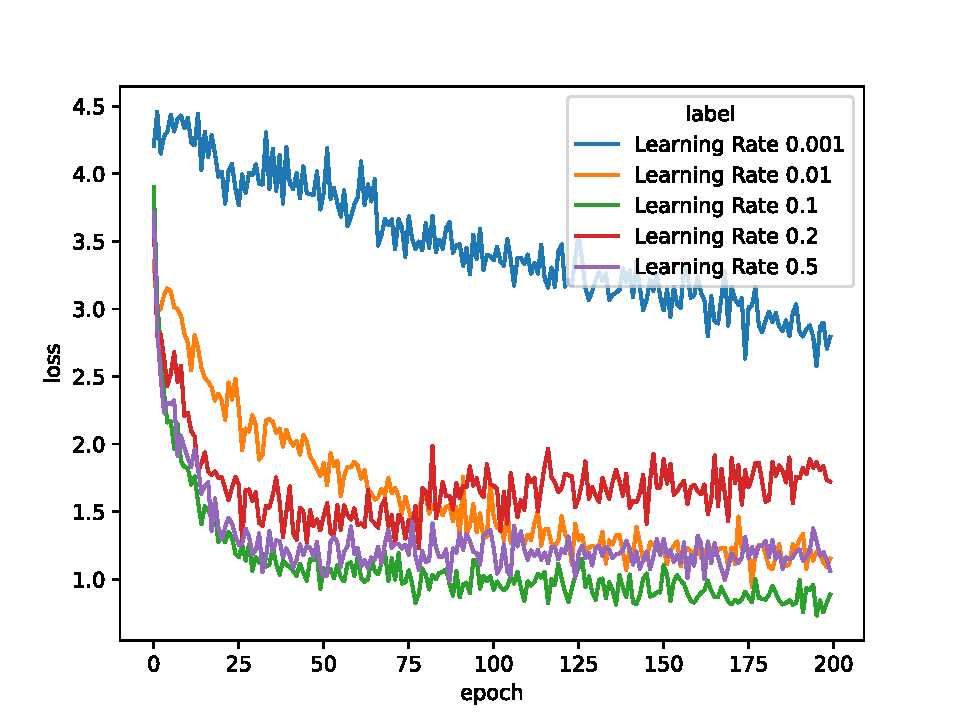
\includegraphics[width=\textwidth]{Node2vec-local}
      \caption{Node2vec-Local}
    \end{subfigure}
    ~
    \begin{subfigure}[b]{0.48\textwidth}
      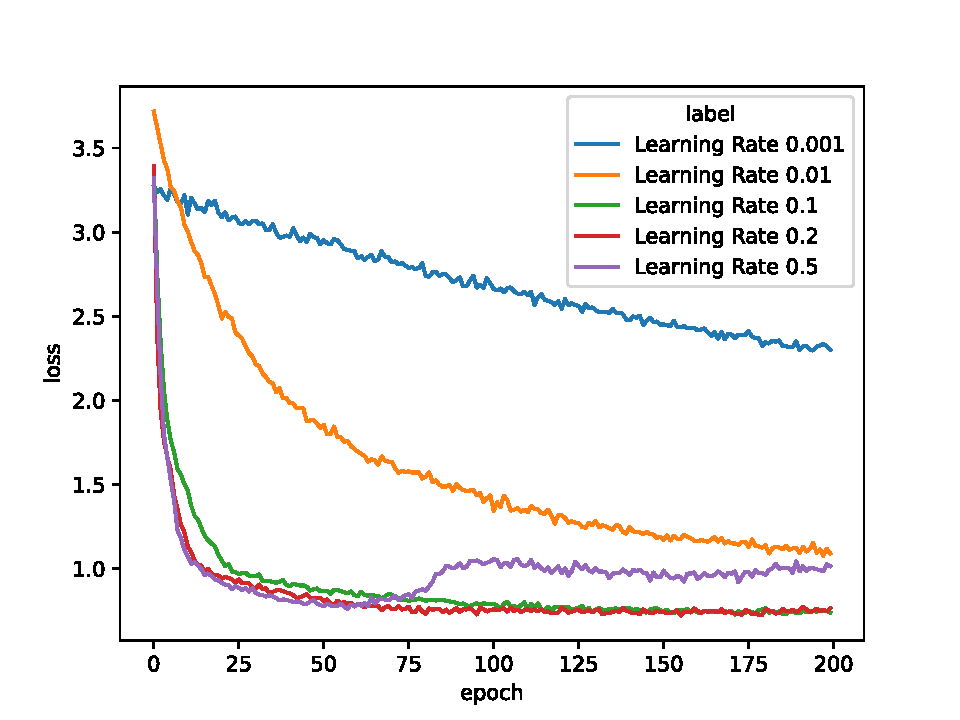
\includegraphics[width=\textwidth]{Node2vec-global}
      \caption{Node2vec-Global}
    \end{subfigure}
    \\
    \begin{subfigure}[b]{0.48\textwidth}
      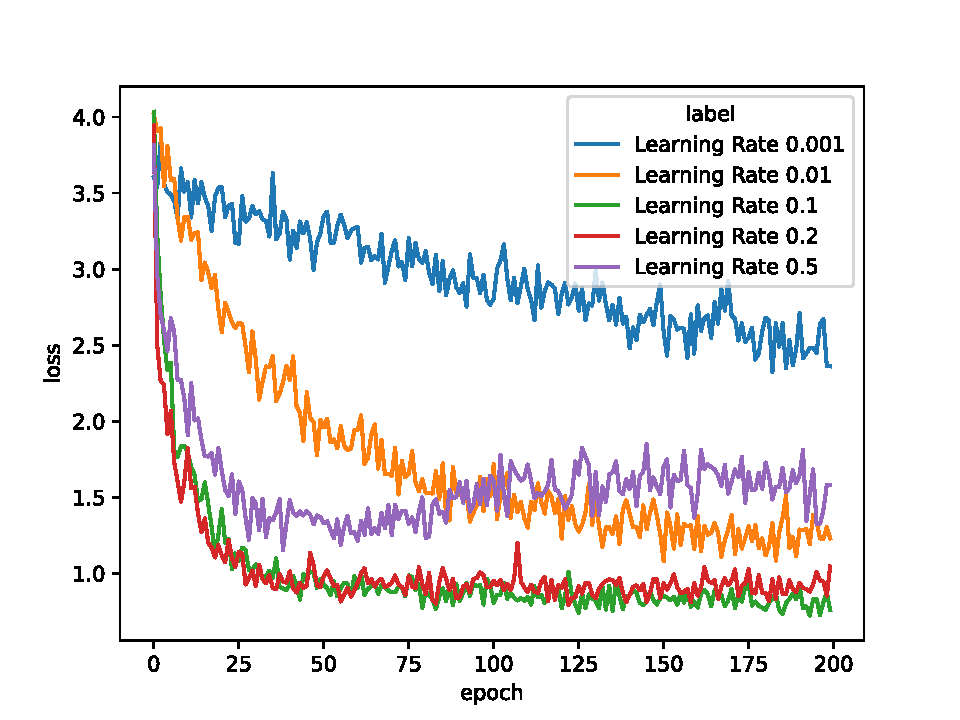
\includegraphics[width=\textwidth]{DeepWalk-local}
      \caption{DeepWalk-Local}
    \end{subfigure}
    ~
    \begin{subfigure}[b]{0.48\textwidth}
      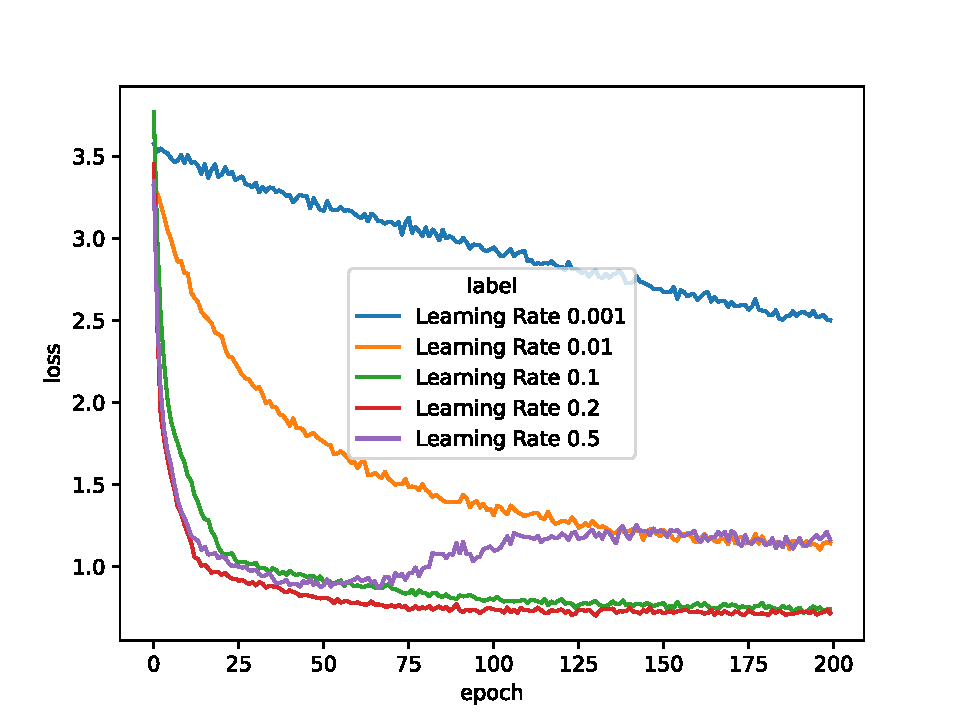
\includegraphics[width=\textwidth]{DeepWalk-global}
      \caption{DeepWalk-Global}
    \end{subfigure}
    \bicaption{\enspace DeepWalk 和 Node2vec 损失函数值与训练轮数曲线图}{\enspace Plots of DeepWalk and Node2vec's loss function values with epoches}
    \label{fig:deep-walk-node2vec}
\end{figure}

对于 GCN、GraphSAGE 和 GAT,本文采用了两个图卷积层,第一个图卷积层采用了 ReLU 激活函数,并有概率为 0.1 的失活(Dropout)层,以避免过拟合;第二个图卷积层采用了 TanH 激活函数。它们的超参数如表~\ref{tab:hyperparameters-gnns}~所示。

\begin{table}[!htbp]
    \bicaption{\enspace GCN、GraphSAGE 和 GAT 的实验超参数设置}{\enspace Hyperparameters of GCN, GraphSAGE and GAT}
    \label{tab:hyperparameters-gnns}
    \centering
    \footnotesize% fontsize
    \setlength{\tabcolsep}{4pt}% column separation
    \renewcommand{\arraystretch}{1.2}%row space 
    \begin{tabular}{ccccccc}
        \hline
        名称 & 模型 & 输入维度 & 隐向量维度 & 输出维度\\
        \hline
        GCN & GCN & 36 & 36 & 36\\
        GraphSAGE & GraphSAGE & 36 & 36 & 36\\
        GAT & GAT & 36 & 36 & 36\\
        \hline
    \end{tabular}
\end{table}

这些模型损失函数值随训练轮数的下降情况如图~\ref{fig:gnns}~所示。可以看出,在图中所示的学习率中,0.01 是三种模型最优的学习率;此外,三种深度图神经网络模型无需只需要很少的迭代就能到达收敛状态。

\begin{figure}[!htbp]
    \centering
    \begin{subfigure}[b]{0.48\textwidth}
      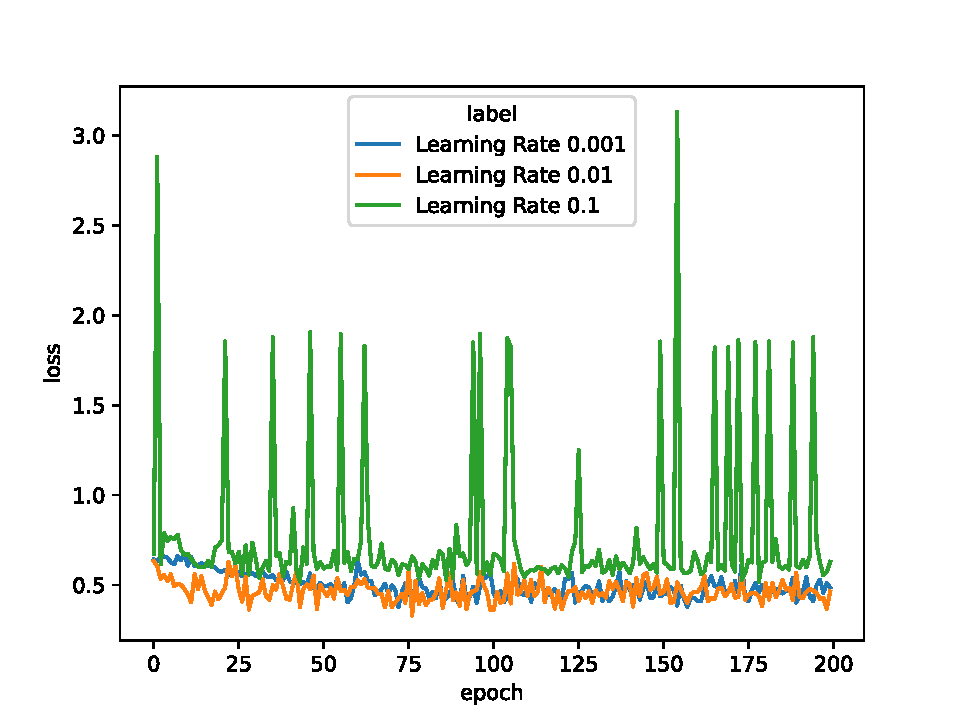
\includegraphics[width=\textwidth]{GCN}
      \caption{GCN}
    \end{subfigure}
    ~
    \begin{subfigure}[b]{0.48\textwidth}
      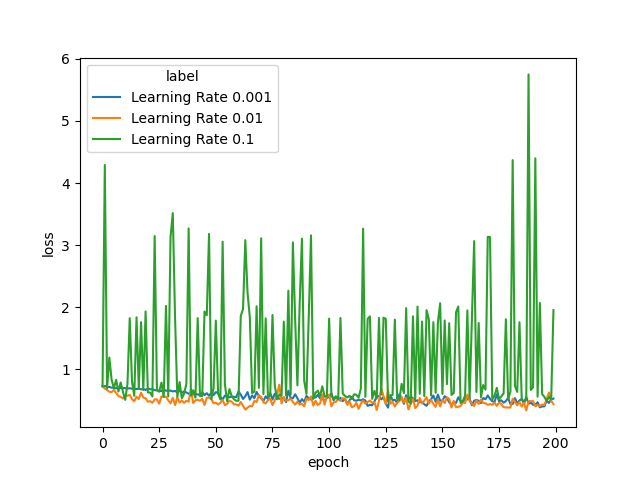
\includegraphics[width=\textwidth]{SAGE}
      \caption{GraphSAGE}
    \end{subfigure}
    \\
    \begin{subfigure}[b]{0.48\textwidth}
      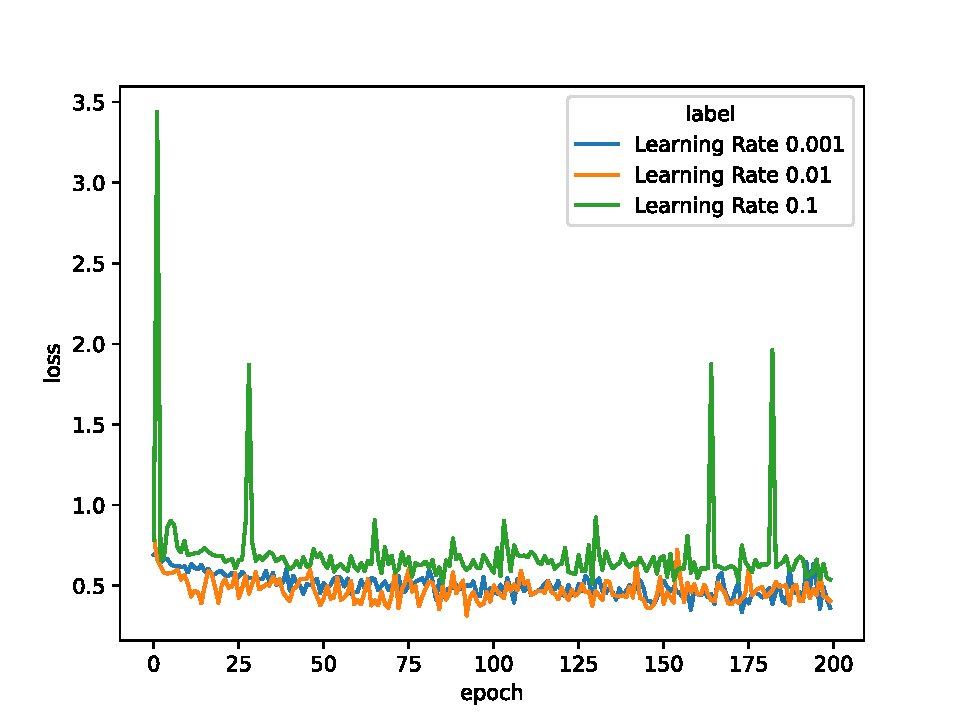
\includegraphics[width=\textwidth]{GAT}
      \caption{GAT}
    \end{subfigure}
    \bicaption{\enspace GCN、GraphSAGE 和 GAT 损失函数值与训练轮数曲线图}{\enspace Plots of GCN, GraphSAGE and GAT's loss function values with epoches}
    \label{fig:gnns}
\end{figure}

最后,取上述五个模型的最佳学习率进行对比,其曲线图如图~\ref{fig:graph-plots}~所示。

\begin{figure}[!htbp]
    \centering
    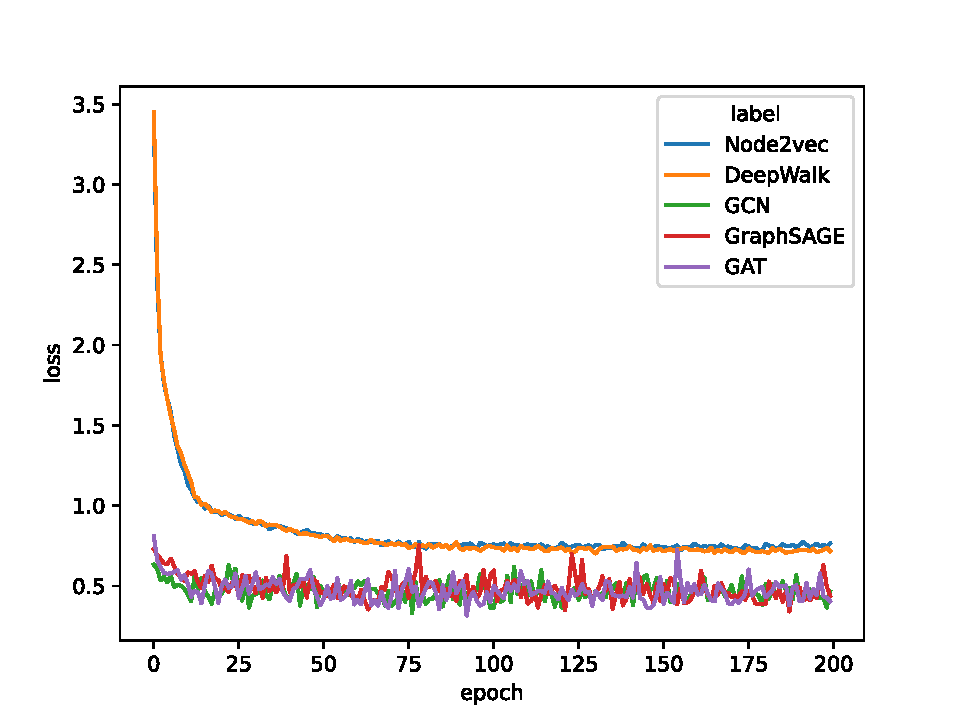
\includegraphics[width=0.48\textwidth]{ALL}
    \bicaption{\enspace 五个图机器学习模型损失函数值与训练轮数曲线图}{\enspace Plots of Five Graph Learning Models' loss function values with epoches}
    \label{fig:graph-plots}
\end{figure}

从图~\ref{fig:graph-plots}~可以看出,在这些机器学习模型中,基于深度学习的模型比基于随机游走的浅层模型收敛更快,这是因为深度学习模型具有更大的容量,有更强的表达能力。在基于深度学习的模型中,三个模型的损失函数值差别不大,但 GCN 模型最为稳定。因此,本文将采用 GCN 模型作为空间特征嵌入方法进行后续的横向移动检测方法研究。

\subsection{时间特征嵌入方法验证}

对于循环神经网络模型 GRU 和 LSTM,本文采用了预测的方式来比较它们的性能,即先将 Kubernetes-dataset 中的良性流量按时间顺序排列后,划分为一定长度的子序列,然后输入至循环神经网络模型中,由循环神经网络模型输出下一时刻的流量预测值,最后取预测值和实际值的欧几里得距离作为模型的评估指标。本文所采用的超参数设置如表~\ref{tab:hyperparameters-rnns}~所示。

\begin{table}[!htbp]
    \bicaption{\enspace GRU 和 LSTM 的实验超参数设置}{\enspace Hyperparameters of GRU and LSTM}
    \label{tab:hyperparameters-rnns}
    \centering
    \footnotesize% fontsize
    \setlength{\tabcolsep}{4pt}% column separation
    \renewcommand{\arraystretch}{1.2}%row space 
    \begin{tabular}{ccccccc}
        \hline
        名称 & 模型 & 层数 & 隐向量维度 & 学习率\\
        \hline
        GRU-1 & GRU & 1 & 同输入流量特征维度 & 0.01\\
        GRU-3 & GRU & 3 & 同输入流量特征维度 & 0.01\\
        LSTM-1 & LSTM & 1 & 同输入流量特征维度 & 0.01\\
        LSTM-3 & LSTM & 3 & 同输入流量特征维度 & 0.01\\
        \hline
    \end{tabular}
\end{table}

其损失函数值随训练轮数的下降情况如图~\ref{fig:rnn-plot}~所示。在这些循环神经网络模型中,三层堆叠的模型比单层堆叠的收敛速度更快,损失函数值更低;与 GRU 相比,LSTM 的预测值更准确,收敛速度也占优势。

\begin{figure}[!htbp]
    \centering
    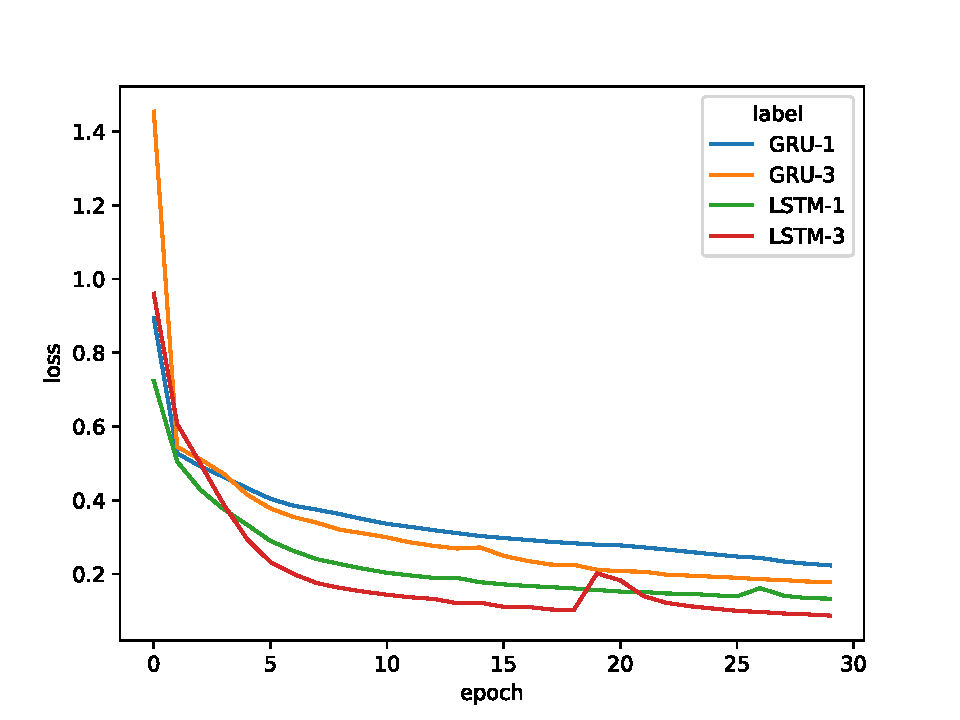
\includegraphics[width=0.48\textwidth]{RNN}
    \bicaption{\enspace GRU 和 LSTM 损失函数值与训练轮数曲线图}{\enspace Plots of GRU and LSTM's loss function values with epoches}
    \label{fig:rnn-plot}
\end{figure}

为了进一步验证四种模型的效果,本文将良性流量的子序列划分为训练集和测试集,其中训练集占比 70\%,测试集占比 30\%。四种模型在测试集上的均方误差如表~\ref{tab:result-rnns}~所示。采用三层 LSTM 的均方误差最低,因此其效果最好。这说明,容量更大的模型具有更强的表达能力。本文将采用三层 LSTM 模型作为时间特征嵌入方法进行后续的横向移动检测模型研究。

\begin{table}[!htbp]
    \bicaption{\enspace GRU 和 LSTM 在测试集上的均方误差结果}{\enspace MSE loss of GRU and LSTM on the test set}
    \label{tab:result-rnns}
    \centering
    \footnotesize% fontsize
    \setlength{\tabcolsep}{4pt}% column separation
    \renewcommand{\arraystretch}{1.2}%row space 
    \begin{tabular}{ccccccc}
        \hline
        名称 & 均方误差\\
        \hline
        GRU-1 & 0.37442\\
        GRU-3 & 0.32283\\
        LSTM-1 & 0.29323\\
        LSTM-3 & 0.28088\\
        \hline
    \end{tabular}
\end{table}

\section{本章小结}

本节首先通过可视化的方式分析容器化集群中网络流量的拓扑结构,对各类通信模式进行了分类,发现了横向移动的关键流。此类流表示一个负载正在攻击者的 C\&C 服务器的控制之下,与 API 服务器进行通信,反映了横向移动攻击的行为。

然而,通过拓扑分析仅能识别出少量的横向移动流量,大部分横向移动流量未能检出。因此,还需要通过机器学习的方法进行识别。本章分析了图神经网络和循环神经网络的多种模型,总结其优缺点,最终选用 GCN 和 LSTM 分别作为时间和空间特征嵌入方法,分别得到各节点的嵌入向量和时间特征向量,供后续模型使用。

}